\section{The BeTSSi submarine model}
\label{Sec3:BeTSSi_description}
In this section the BeTSSi \cite{Nolte2014bib} submarine model (depicted in \Cref{Fig3:BeTSSi_BC}) will be presented. The BeTSSi submarine contains many standard designing features including circles, ellipses, straight panels, cylinders and cones. In addition, several NACA profiles are present giving a very nice benchmark model for sub-surface scattering. For the analysis part, it contains challenges such as trimming curves and non-Lipschitz domains~\cite{Lipton2010roi}. All in all, a challenging benchmark without being too complex.
\begin{figure}
	\centering
	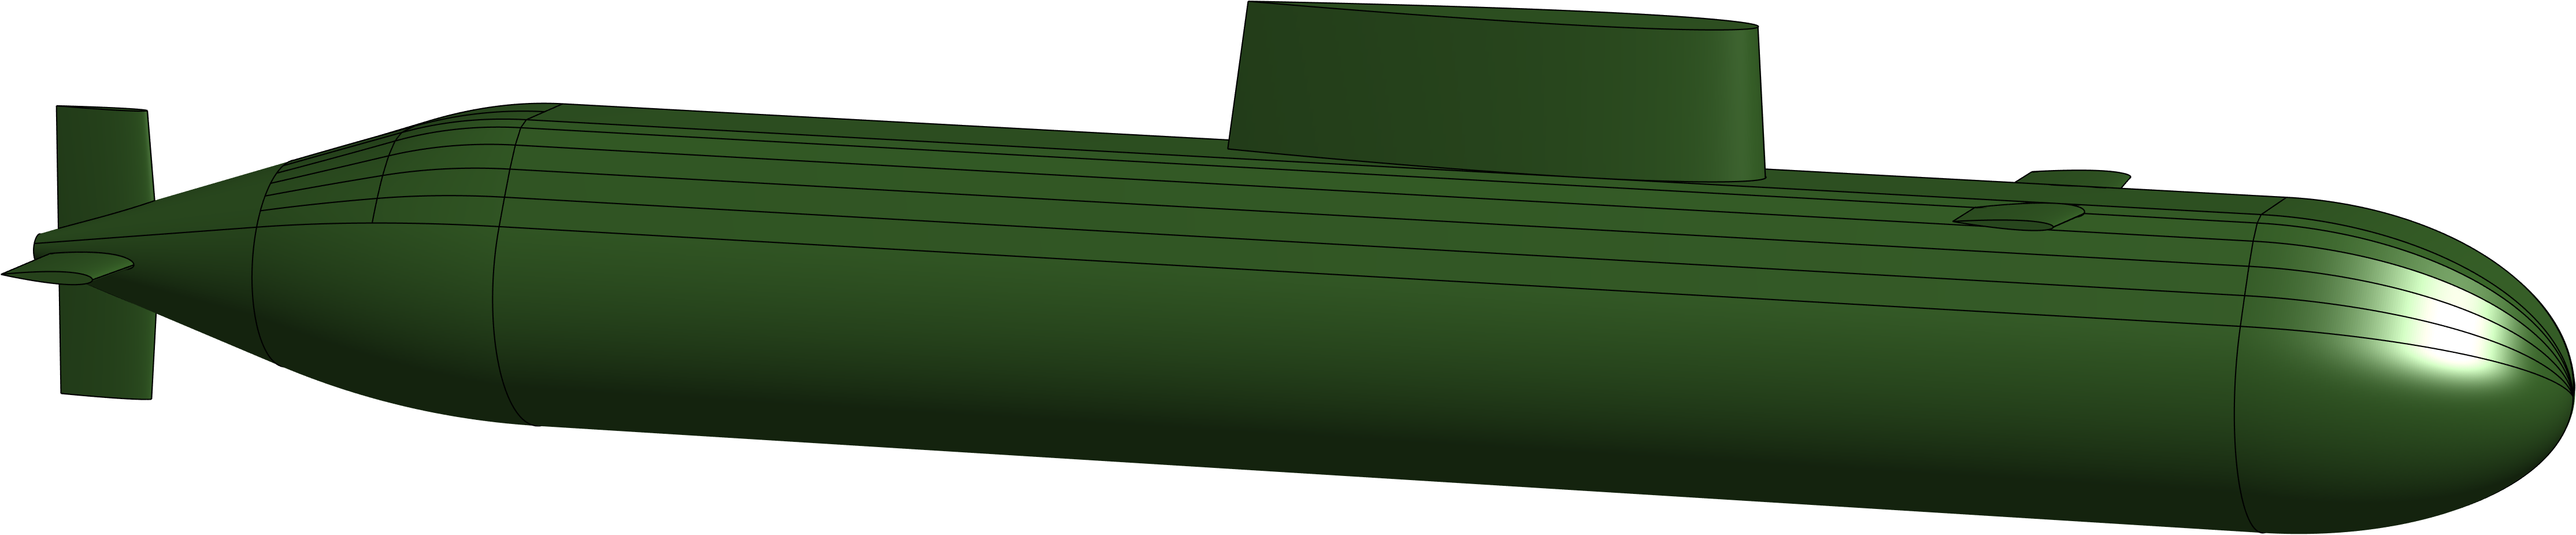
\includegraphics[width=\textwidth]{CAD}
	\caption{Outer pressure hull for BeTSSi submarine.}
	\label{Fig3:BeTSSi_BC}
\end{figure}

The original BeTSSi submarine model presented in  \cite{Nolte2014bib} contains several discrepancies that is arguably not optimal for a benchmark model. First, the NACA profiles used to create the sail and the rudders are only given with 5 digits of accuracy. This in turn, results in for example the sail not being tangent to the side lines of the deck with an error of around $\SI{1}{mm}$. This creates problems for the meshing procedure as this results in either very small elements in this area, or element with high aspect ratios. Second, the exact geometry for the upper transition from the deck to the rotationally symmetric cone tail, is hidden by an ``internal routine in ANSYS''. Not only is this hard to reproduce for anyone without an ANSYS license, but the available CAD file for this model does not represent the transition to the lower part exactly (as this curve should be a circular arc and is not represented by a NURBS curve). In order to create a watertight model, the available CAD file approximates the lower transition such that the side curves match. 

The relevant BeTSSi parameters for the work presented herein are given in \Cref{Tab3:BeTSSiParameters}.
\begin{table}
	\centering
	\caption{\textbf{BeTSSi submarine:} Free parameters for the BeTSSi submarine benchmark.}
	\label{Tab3:BeTSSiParameters}
	\begin{tabular}{l l}
		\toprule
		Parameter & Description\\
		\midrule
		$\alpha=\ang{18}$ & Arc angle of transition to the tail cone\\
		$\beta=\ang{240}$ & Rotational angle for the axisymmetric lower part\\
		$g_2=\SI{6.5}{m}$ & Distance in the $x$-direction of transition to the tail cone\\
		$g_3=\SI{6.5}{m}$ & Distance in the $x$-direction of the tail cone\\
		$L=\SI{42}{m}$ & Length of the deck\\
		$a=\SI{7}{m}$ & Semi-major axis of bow\\
		$b=\SI{3.5}{m}$ & Semi-minor axis of bow\\
		$c=\SI{4}{m}$ & Height from the $x$-axis to the deck\\
		$s=\SI{1.2}{m}$ & Half of the width of the deck\\
		$l_{\mathrm{ls}}=\SI{13}{m}$ & Length of the lower cross-section of the sail\\
		$l_{\mathrm{lm}}=\SI{2.6}{m}$ & Length of the lower cross-section of the main rudders\\
		$l_{\mathrm{ld}}=\SI{2.6}{m}$ & Length of the lower cross-section of the depth rudders\\
		$l_{\mathrm{us}}=\SI{12.3}{m}$ & Length of the upper cross-section of the sail\\
		$l_{\mathrm{um}}=\SI{2.35}{m}$ & Length of the upper cross-section of the main rudders\\
		$l_{\mathrm{ud}}=\SI{2.35}{m}$ & Length of the upper cross-section of the depth rudders\\
		$b_{\mathrm{lm}}=\SI{0.4}{m}$ & Width of the lower cross-section of the main rudders\\
		$b_{\mathrm{us}}=\SI{2}{m}$ & Width of the upper cross-section of the sail\\
		$b_{\mathrm{um}}=\SI{0.3}{m}$ & Width of the upper cross-section of the main rudders\\
		$b_{\mathrm{ud}}=\SI{0.22}{m}$ & Width of the upper cross-section of the depth rudders\\
		$\delta_{\mathrm{s}}=\SI{0.2}{m}$ & Parameter for shifting cross-sections of the sail\\
		$h_{\mathrm{s}}=\SI{3.5}{m}$ & Height of the sail\\
		$h_{\mathrm{m}}=\SI{3.5}{m}$ & Height of the main rudders\\
		$x_{\mathrm{s}}=-\SI{12}{m}$ & Positioning of the sail\\
		$x_{\mathrm{m}}=-\SI{51.9}{m}$ & Positioning of the main rudders\\
		$x_{\mathrm{d}}=-\SI{4}{m}$ & Positioning of the depth rudders\\
		\bottomrule
	\end{tabular}
\end{table}

\subsection{Main body}
The model is symmetric about the $xz$-plane and has rotational symmetry for the lower part as described in \Cref{Fig3:bettsi_bottom}.
\begin{figure}
	\centering
	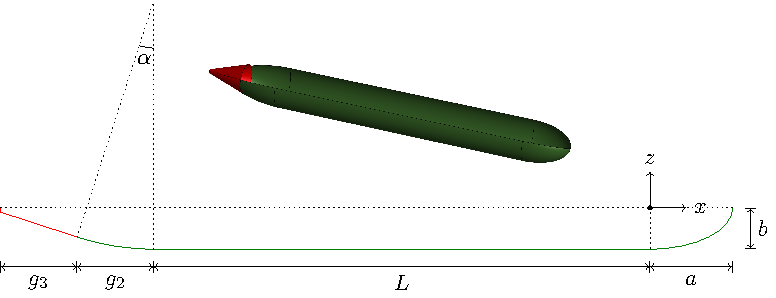
\includegraphics[scale=1]{betssi_bottom}
	\caption{The sideline of the lower part of the BeTSSi submarine. The side lines are formed (from the right) by an ellipse with semi-major axis $a$ and semi-minor axis $b$, followed by a straight line of length $L$, then an arc of angle $\alpha$ and finally two straight lines. The latter two straight lines (in red) are rotated about the $x$-axis and the remaining part (in green) are rotated an angle $\beta$ around the $x$-axis.}
	\label{Fig3:bettsi_bottom}
\end{figure}
The transition from this axisymmetric part to the deck is described in \Cref{Fig3:bettsi_top}. This transition as well as the deck itself, contains a set of rectangular panels of length $L$.
\begin{figure}
	\centering
	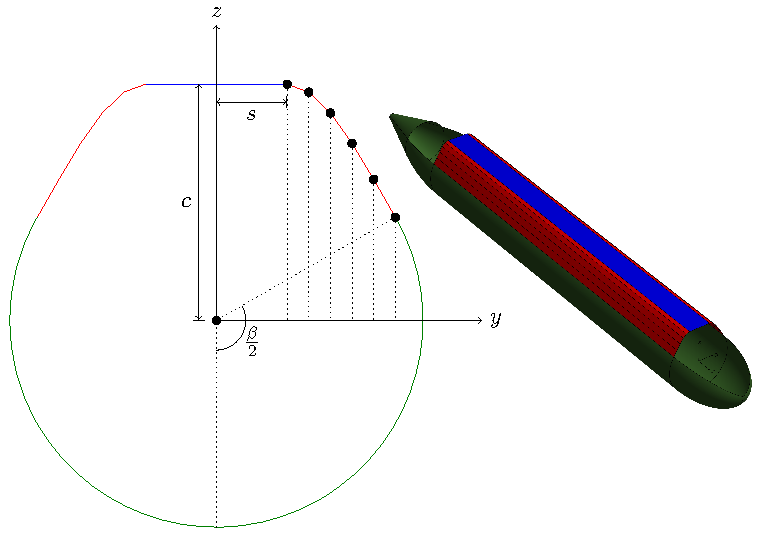
\includegraphics[scale=1]{betssi_top}
	\caption{The transition (red line) from the axisymmetric hull (green line) to the deck (blue line) is given by sampling a cubic polynomial, $P_{\mathrm{p}}(y)$, at 6 equidistant points in the $y$-direction and connecting the resulting points with straight lines (corresponding 6 points are found for negative values $y$-values, $(0,y,P_{\mathrm{p}}(|y|))$).}
	\label{Fig3:bettsi_top}
\end{figure}
The cubic polynomial $P_{\mathrm{p}}(y)$, is uniquely defined by the requirement that it defines a smooth transition between the hull and the deck. More precisely, the following requirement must be satisfied: 
\begin{alignat*}{3}
	P_{\mathrm{p}}(s) &= c,\quad  &&P_{\mathrm{p}}\left(b\sin\frac{\beta}{2}\right) = -b\cos\frac{\beta}{2}\\
	P_{\mathrm{p}}'(s) &= 0,\quad &&P_{\mathrm{p}}'\left(b\sin\frac{\beta}{2}\right) = \tan\frac{\beta}{2}
\end{alignat*}
which gives the polynomial
\begin{equation*}
	P_{\mathrm{p}}(y) = c+C_1(y-s)^2+C_2(y-s)^3
\end{equation*}
where
\begin{equation*}
\begin{aligned}
	&C_1 = -\frac{3C_4+C_3\tan\frac{\beta}{2}}{C_3^2}, \quad
	C_2 = \frac{2C_4+C_3\tan\frac{\beta}{2}}{C_3^3}\\
	&C_3 = b\sin\frac{\beta}{2}-s, \quad
	C_4 = c+b\cos\frac{\beta}{2}.
\end{aligned}
\end{equation*}
The upper part of the bow (highlighted in \Cref{Fig3:bettsi_upperBow}) is obtained by linear lofting of elliptic curves from the 12 points described in \Cref{Fig3:bettsi_top} to the tip of the bow. 

The upper part of the tail section (highlighted in \Cref{Fig3:bettsi_upperPartOfTailSection}) is connected using a tensor NURBS surface of degree 2 such that it defines a smooth transition from the axisymmetric cone to the deck. More precisely, the upper part of the cone tail is divided into 12 arcs with angle $\frac{2\PI-\beta}{12}$, and the resulting points are connected to corresponding points on the transition to the deck from the axisymmetric hull. 
\begin{figure}
	\centering    
	\begin{subfigure}{0.49\textwidth}
		\centering
		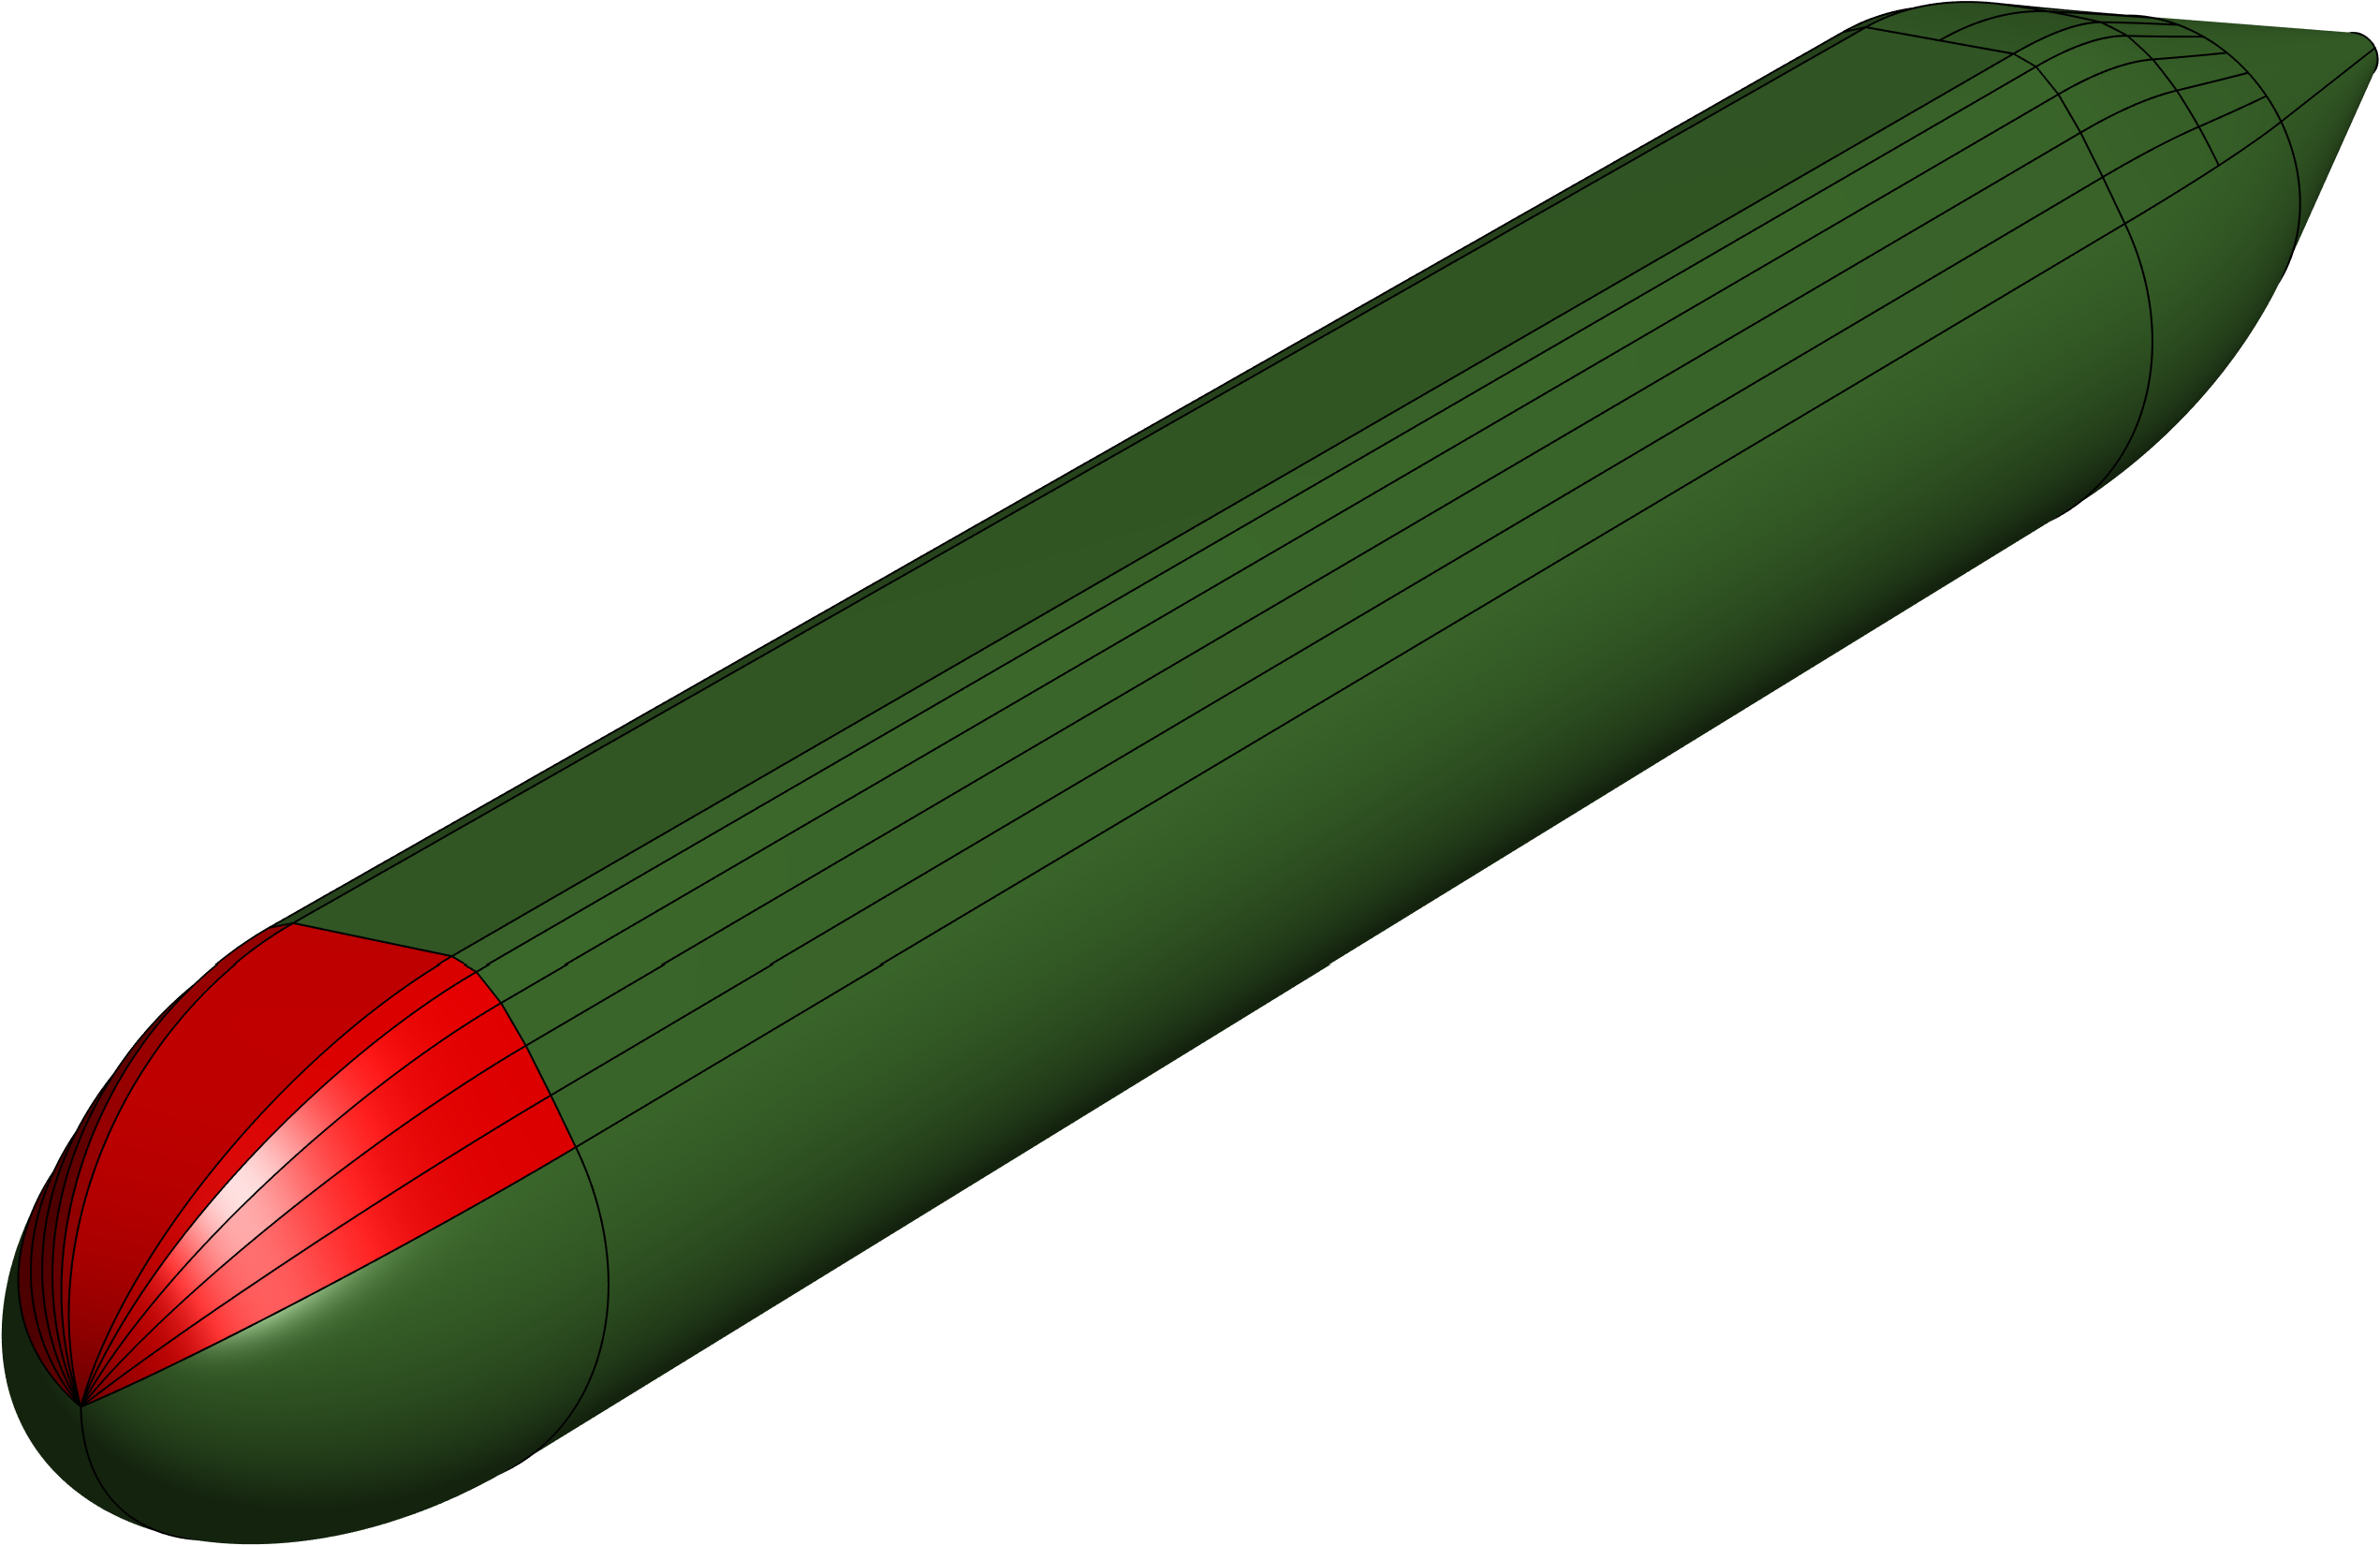
\includegraphics[width=\textwidth]{CAD_bow}
		\caption{Illustration of the upper bow part.}
		\label{Fig3:bettsi_upperBow}
	\end{subfigure}%
	\hspace*{0.02\textwidth}%  
	\begin{subfigure}{0.49\textwidth}
		\centering
		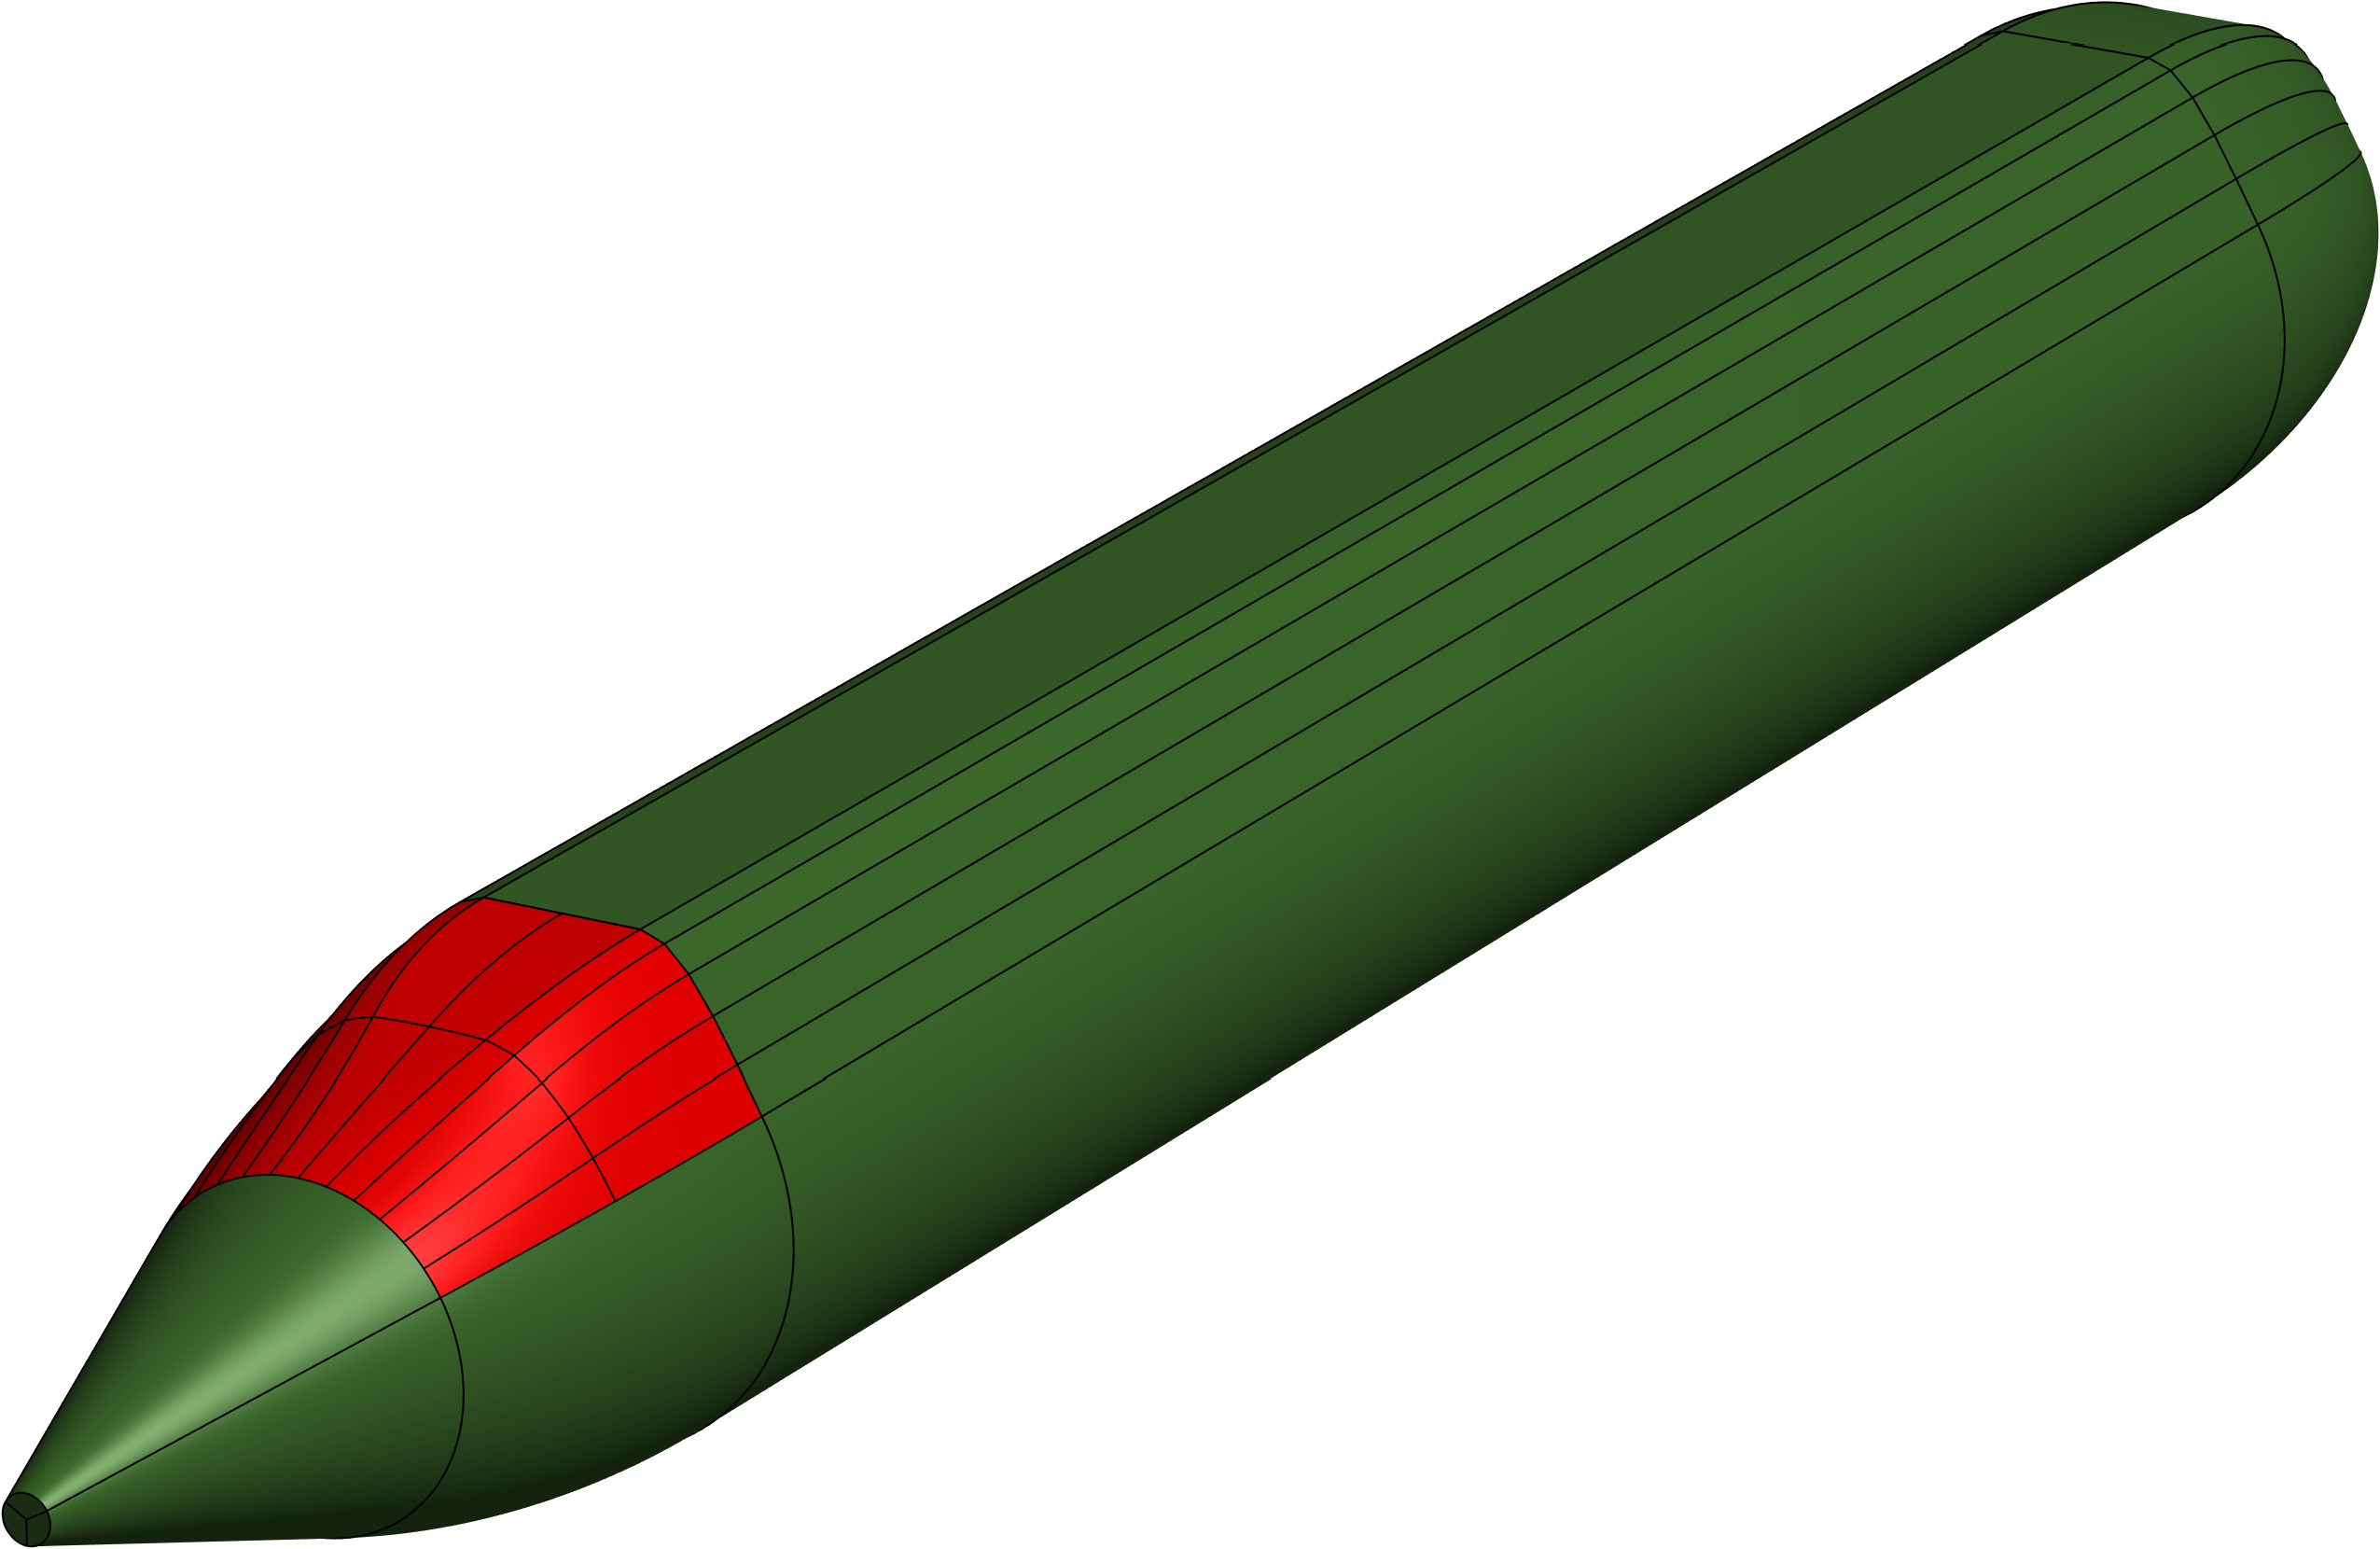
\includegraphics[width=\textwidth]{CAD_transition}
		\caption{Illustration of the upper transition part.}
		\label{Fig3:bettsi_upperPartOfTailSection}
	\end{subfigure}
	\caption{Main body of BeTSSi submarine.}
\end{figure}
As illustrated in \Cref{Fig3:BeTSSi_BC_tailSection}, the NURBS patch is given by 24 elements. Thus, $4\cdot 25 = 100$ control points, $\vec{P}_{i,j}$, are needed as shown in \Cref{Fig3:BeTSSi_BC_tailSection_cp} (25 and 4 control points in the $\xi$ direction and $\eta$ direction, respectively).
\begin{figure}
	\centering    
	\begin{subfigure}{0.49\textwidth}
		\centering
		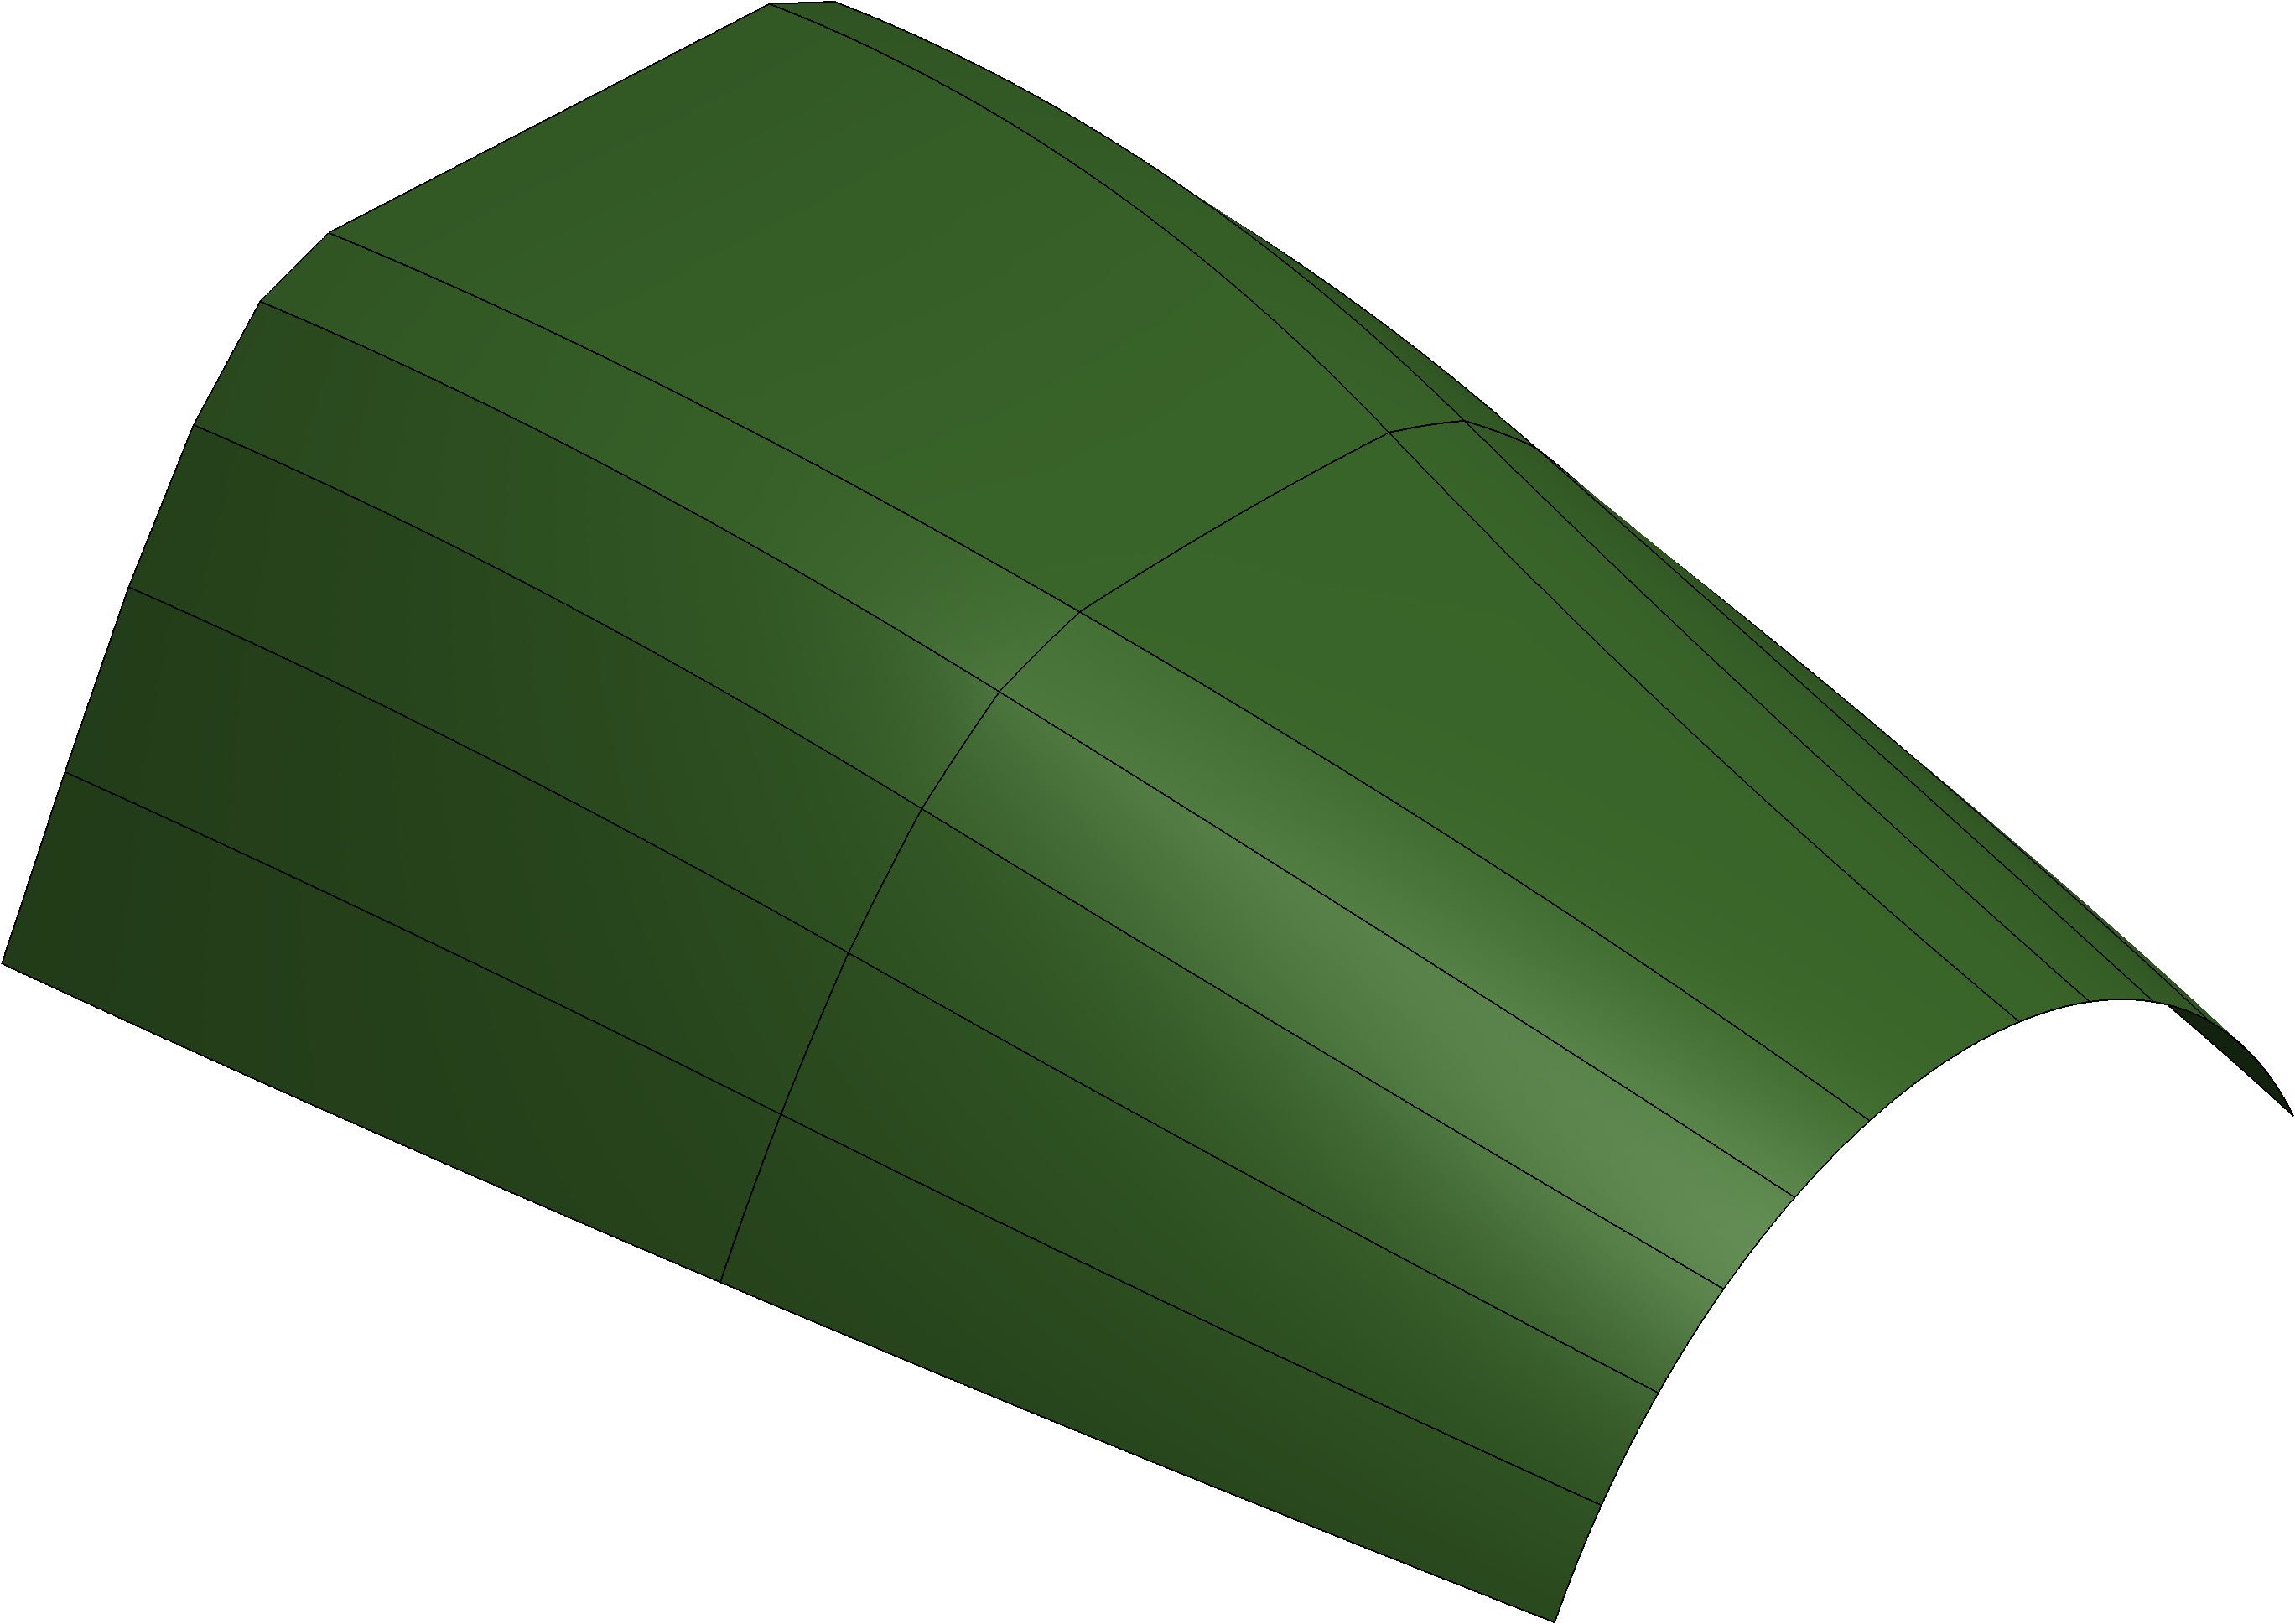
\includegraphics[width=0.9\textwidth]{BeTSSi_BC_tailSection}
		\caption{Illustration of the mesh.}
		\label{Fig3:BeTSSi_BC_tailSection}
	\end{subfigure}%
	\hspace*{0.02\textwidth}%  
	\begin{subfigure}{0.49\textwidth}
		\centering
		\includegraphics{tailSectionNEW}
		\caption{Illustration of the control polygon mesh.}
		\label{Fig3:BeTSSi_BC_tailSection_cp}
	\end{subfigure}
	\caption{Illustration of the upper transition part of the tail.}
\end{figure}
The control points $\vec{P}_{1,j}$ and $\vec{P}_{25,j}$ for $j=1,2,3,4$ must be defined as in \Cref{Fig3:arcParam2}, while the control points $\vec{P}_{i,1}$ must be defined as in \Cref{Fig3:arcParam1}. The weights are defined by
\begin{equation*}
	w_{i,j} = \begin{cases}
		\tilde{w}_j & i\,\, \text{odd}\\
		\frac{\tilde{w}_j}{3}\left[(4-j)\cos\left(\frac{2\PI-\beta}{24}\right)+j-1\right] & i\,\, \text{even}
		\end{cases}		
\end{equation*}
where
\begin{equation*}
	\tilde{w}_j = \begin{cases}
		1 & j = 1,4\\
		\frac{1}{2}\left(1+\cos\frac{\alpha}{2}\right) & j = 2,3.
	\end{cases}
\end{equation*}
The locations of the control points $\vec{P}_{i,j}$, $j=2,3$ and $2\leq i\leq 24$, are determined by the requirement that the $x$ component is the same as $\vec{P}_{1,j}$ and the fact that the control polygon lines must be tangential to the surface both at the deck and the cone tail.
\begin{figure}
	\centering    
	\begin{subfigure}{0.44\textwidth}
		\centering
		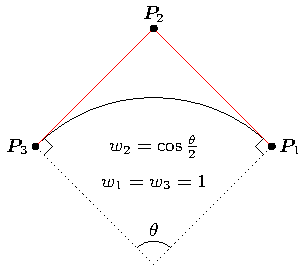
\includegraphics{knotInsertionArc_1}
		\caption{NURBS parametrization of arc of angle $\theta$ using three control points $\{\vec{P}_i\}_{i=1}^3$, the weights $\{w_i\}_{i=1}^3$ and the open knot vector $\Xi=\{0,0,0,1,1,1\}$.}
		\label{Fig3:arcParam1}
	\end{subfigure}%
	\hspace*{0.02\textwidth}%  
	\begin{subfigure}{0.54\textwidth}
		\centering
		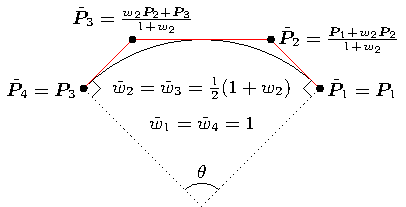
\includegraphics{knotInsertionArc_2}
		\caption{NURBS parametrization of arc of angle $\theta$ using four control points $\{\tilde{\vec{P}}_i\}_{i=1}^4$, the weights $\{\tilde{w}_i\}_{i=1}^4$ and the open knot vector $\tilde{\vec{t}}_\upxi=\{0,0,0,0.5,1,1,1\}$.}
		\label{Fig3:arcParam2}
	\end{subfigure}
	\caption{Two ways of parametrizing an arc using NURBS~\cite[p. 315]{Piegl1997tnb}.}
\end{figure}

\subsection{NACA profiles}
The sail and the rudders are based on the NACA 00xx profiles \cite{Ladson1996cpt,Cummings2015gfa} (the first two digits indicate a symmetric airfoil, and the second two, the thickness-chord ratio). The NACA profiles are all based on the function
\begin{equation}\label{Eq3:NACA}
	f_t(x) = 5t\left(a_0\sqrt{x} + a_1x +a_2x^2+a_3x^3+a_4x^4\right)
\end{equation}
with $t$ being the thickness of the rudder and $a_i$ the coefficients determining the shape of the rudder.

This function satisfies the condition $f_t(0)=0$ and should in addition satisfy
\begin{equation}\label{Eq3:NACAmainConditions}
	f_t(0.3) = \frac{t}{2}, \quad f_t'(0.3) = 0.
\end{equation}
In \cite{Ladson1996cpt,Cummings2015gfa} the coefficients are computed to be
\begin{align*}
	a_0 &= 0.2969\\
	a_1 &=-0.1260\\
	a_2 &=-0.3516\\
	a_3 &= 0.2843\\
	a_4 &=-0.1015.
\end{align*}
The conditions in \Cref{Eq3:NACAmainConditions} are approximated with a residual error of 0.0029\% and 0.013\%, respectively. Moreover, the additional condition $f_t(1) = 0.002$ is satisfied with a  residual error of 0.01\%. In order to have a zero-thickness trailing edge, i.e. $f_t(1)=0$, the original BeTSSi coefficients slightly modify the NACA coefficients to be
\begin{align*}
	a_0 &= 0.2969\\
	a_1 &=-0.1267\\
	a_2 &=-0.3523\\
	a_3 &= 0.2843\\
	a_4 &=-0.1022.
\end{align*}
The conditions in \Cref{Eq3:NACAmainConditions} are here approximated with a residual error of 0.025\% and 0.013\%, respectively. The fact that the conditions in \Cref{Eq3:NACAmainConditions} are approximated so poorly is problematic for an analysis suitable BeTSSi submarine as this results in tangential curves missing the NACA profiles with a significant error, resulting in elements with high aspect ratio or a redundant amount of elements in order to resolve these areas. This fact motivates a more precise definition of these coefficients.

Note that the leading-edge radius is given by
\begin{equation*}
	R_{\mathrm{le}} =\lim_{x\to 0^+} \left|\frac{\left[1+f_t'(x)^2\right]^{3/2}}{f_t''(x)}\right| =  \frac{25}{2}a_0^2t^2
\end{equation*}
and the included angle of the trailing edge by
\begin{equation*}
	\delta_{\mathrm{te}} = 2\tan^{-1}|f_t'(1)|.
\end{equation*}
Alternative conditions \cite{Cummings2015gfa}
\begin{equation}\label{Eq3:NACAconditions2}
	R_{\mathrm{le}} = \frac{25}{2}0.2969^2t^2,\quad \delta_{\mathrm{te}} = 2\tan^{-1}(5t\cdot 0.23385)
\end{equation}
yield the coefficients (for usage in double precision)
\begin{align*}
	a_0 &= 0.2969\\
	a_1 &\approx-0.128361732706295\\
	a_2 &\approx-0.335670924960620\\
	a_3 &\approx 0.251127048040123\\
	a_4 &\approx-0.083994390373209.
\end{align*}
Using
\begin{equation*}
	\delta_{\mathrm{te}} = 2\tan^{-1}(5t\cdot 0.243895)
\end{equation*}
yields coefficients slightly closer to the original BeTSSi coefficients.

In summary, we shall use the conditions
\begin{equation}\label{Eq3:NACAconditions3}
	f_t(1) = 0,\quad  f_t(0.3) = \frac{t}{2}, \quad f_t'(0.3) = 0,\quad a_0 = 0.2969,\quad f_t'(1) = -5 t\cdot 0.243895
\end{equation}
which are illustrated in \Cref{Fig3:NACA2} and yields the coefficients (in double precision)
\begin{align*}
	a_0 &= 0.2969\\
	a_1 &\approx-0.12651673270629464\\
	a_2 &\approx-0.34981592496061949\\
	a_3 &\approx 0.28392704804012290\\
	a_4 &\approx-0.10449439037320877.
\end{align*}

\begin{figure}
	\centering
	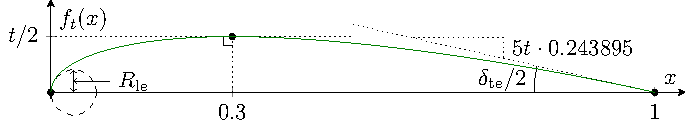
\includegraphics{NACA2}
	\caption{Illustration of the NACA profile used for the sail and the rudders. The five coefficients $a_i$ in \Cref{Eq3:NACA} are restricted by the conditions in \Cref{Eq3:NACAconditions3} as illustrated here.}
	\label{Fig3:NACA2}
\end{figure}
Computing the relative error in the $L^2$-norm of the NACA profile based on these coefficients and the original NACA profile for the BeTSSi submarine yields an error of about $0.54\%$. Note that $f_t(\xi^2)$ is a polynomial of degree 8, such that the NACA profile can be exactly represented by a spline curve based on the parametrization $\vec{C}(\xi) = [\xi^2,f_t(\xi^2)]$. 

\subsection{Sail}
Consider the port part ($y\geq 0$) of the sail. It can be parametrized by
\begin{equation}\label{Eq3:sail}
	\vec{S}_{\mathrm{s}}(\xi,\eta) = x_{\mathrm{s}}\vec{e}_{\mathrm{x}} + c\vec{e}_{\mathrm{z}} + \begin{bmatrix}
	-\left[l_{\mathrm{ls}} \xi^2+\eta\left(\delta_{\mathrm{s}}-(l_{\mathrm{ls}}-l_{\mathrm{us}})\xi^2\right)\right]\\
	l_{\mathrm{ls}}f_{t_{\mathrm{ls}}}(\xi^2) + \eta\left[l_{\mathrm{us}}f_{t_{\mathrm{us}}}(\xi^2)-l_{\mathrm{ls}}f_{t_{\mathrm{ls}}}(\xi^2)\right]\\
	\eta h_{\mathrm{s}}
	\end{bmatrix}
\end{equation}
where
\begin{equation*}
	0\leq \xi\leq 1,\quad 0\leq \eta \leq 1,\quad t_{\mathrm{us}}=\frac{b_{\mathrm{us}}}{l_{\mathrm{us}}},\quad t_{\mathrm{ls}}=\frac{b_{\mathrm{ls}}}{l_{\mathrm{ls}}},\quad\text{and}\quad b_{\mathrm{ls}}=2s.
\end{equation*}
This parametrization is illustrated in \Cref{Fig3:rudders}. The starboard part of the sail is obtained by mirroring the port side of the sail about the $xz$-plane. Finally, the roof is obtained by a linear loft between these two surfaces.
\begin{figure}
	\centering
	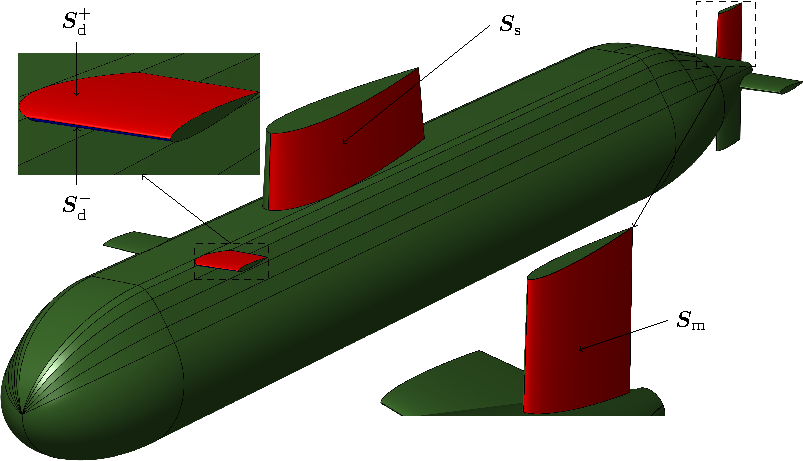
\includegraphics{rudders}
	\caption{Illustration of the parametrizations $\vec{S}_{\mathrm{s}}$, $\vec{S}_{\mathrm{m}}$ and $\vec{S}_{\mathrm{d}}^\pm$ for the sail, the main rudders and the depth rudders, respectively.}
	\label{Fig3:rudders}
\end{figure}

\subsection{Main rudders}
Consider the port part ($y\geq 0$) of the upper main rudder. It can be parametrized by
\begin{equation}\label{Eq3:mainRudders}
	\vec{S}_{\mathrm{m}}(\xi,\eta) = x_{\mathrm{m}}\vec{e}_{\mathrm{x}} + \begin{bmatrix}
	-l_{\mathrm{lm}} \xi^2-\delta_{\mathrm{m}}\eta\left(1-\xi^2\right)\\
	l_{\mathrm{lm}}f_{t_{\mathrm{lm}}}(\xi^2) + \eta\left[l_{\mathrm{um}}f_{t_{\mathrm{um}}}(\xi^2)-l_{\mathrm{lm}}f_{t_{\mathrm{lm}}}(\xi^2)\right]\\
	\eta h_{\mathrm{m}}
	\end{bmatrix}, 
\end{equation}
where
\begin{equation*}
	0\leq \xi\leq 1,\quad g(\xi)\leq \eta \leq 1,\quad\delta_{\mathrm{m}}=l_{\mathrm{lm}}-l_{\mathrm{um}},\quad t_{\mathrm{lm}}=\frac{b_{\mathrm{lm}}}{l_{\mathrm{lm}}},\quad\text{and}\quad t_{\mathrm{um}}=\frac{b_{\mathrm{um}}}{l_{\mathrm{um}}}
\end{equation*}
for a function $g$ (to be determined) representing the intersection between the rudder and the cone. The cone can be represented by
\begin{equation}\label{Eq3:cone}
	y^2+z^2=\left(x-x_{\mathrm{c}}\right)^2\tan^2\alpha,\quad x_{\mathrm{c}} = -(L+g_2+(b-h)\cot\alpha).
\end{equation}
Then, inserting the components of $\vec{S}_{\mathrm{m}}(\xi,\eta)$ in \Cref{Eq3:mainRudders} into \Cref{Eq3:cone} yields an equation in $\xi$ and $\eta$. This equation is quadratic in $\eta$ and has the solution $\eta=g(\xi)$ where
\begin{equation*}
	g(\xi) = \frac{-C_{\mathrm{b}}(\xi) + \sqrt{[C_{\mathrm{b}}(\xi)]^2-4C_{\mathrm{a}}(\xi)C_{\mathrm{c}}(\xi)}}{2C_{\mathrm{a}}(\xi)}
\end{equation*}
and
\begin{align*}
	C_{\mathrm{a}}(\xi) &= \left[l_{\mathrm{um}}f_{t_{\mathrm{um}}}(\xi^2)-l_{\mathrm{lm}}f_{t_{\mathrm{lm}}}(\xi^2)\right]^2+h_{\mathrm{m}}^2-\delta_{\mathrm{m}}^2(1-\xi^2)^2\tan^2\alpha\\
	C_{\mathrm{b}}(\xi) &= 2l_{\mathrm{lm}}f_{t_{\mathrm{lm}}}(\xi^2)\left[l_{\mathrm{um}}f_{t_{\mathrm{um}}}(\xi^2)-l_{\mathrm{lm}}f_{t_{\mathrm{lm}}}(\xi^2)\right]\\
	&\quad+2\tan^2\alpha\left(x_{\mathrm{m}}-l_{\mathrm{lm}}\xi^2-x_{\mathrm{c}}\right)\delta_{\mathrm{m}}\left(1-\xi^2\right)\\
	C_{\mathrm{c}}(\xi) &= [l_{\mathrm{lm}}f_{t_{\mathrm{lm}}}(\xi^2)]^2 - \tan^2\alpha\left(x_{\mathrm{m}}-l_{\mathrm{lm}}\xi^2-x_{\mathrm{c}}\right)^2.
\end{align*}
The trimming curve is then given by
\begin{equation*}
	\vec{r}_{\mathrm{m}}(\xi) = \vec{S}_{\mathrm{m}}(\xi,g(\xi)).
\end{equation*}
The parametrization $\vec{S}_{\mathrm{m}}$ is illustrated in \Cref{Fig3:rudders}. The starboard side of the upper main rudder is given by mirroring the port side of the main upper rudder about the $xz$-plane, and the top part of the rudder is connected by linear lofting. The other main rudders are obtained by rotations by angles of $\ang{90}$, $\ang{180}$ and $\ang{270}$ around the $x$-axis, respectively. Note that this trimming curve may not be represented exactly by NURBS basis functions, and hence, the BeTSSi submarine cannot be exactly represented by NURBS patches without trimming curves.

\subsection{Depth rudders}
Consider the port depth rudder ($y\geq 0$). The upper ($+$) part and lower ($-$) part can be parametrized by
\begin{equation}\label{Eq3:depthRudders}
	\vec{S}_{\mathrm{d}}^\pm(\xi,\eta) = \begin{bmatrix}
		x_{\mathrm{d}}\\
		s\\
		c-\frac{b_{\mathrm{ld}}}{2}
\end{bmatrix}	 + \begin{bmatrix}
	-l_{\mathrm{ld}} \xi^2-\delta_{\mathrm{d}}\eta\left(1-\xi^2\right)\\
	\eta h_{\mathrm{d}}\\
	\pm l_{\mathrm{ld}}f_{t_{\mathrm{ld}}}(\xi^2) \pm \eta\left[l_{\mathrm{ud}}f_{t_{\mathrm{ud}}}(\xi^2)-l_{\mathrm{ld}}f_{t_{\mathrm{ld}}}(\xi^2)\right]
	\end{bmatrix},
\end{equation}
where
\begin{equation*}
\begin{aligned}
	0\leq \xi\leq 1,\quad g^\pm(\xi)\leq \eta \leq 1,
	\delta_{\mathrm{d}}=l_{\mathrm{ld}}-l_{\mathrm{ud}},\quad t_{\mathrm{ld}}=\frac{b_{\mathrm{ld}}}{l_{\mathrm{ld}}},\quad t_{\mathrm{ud}}=\frac{b_{\mathrm{ud}}}{l_{\mathrm{ud}}},\\
	h_{\mathrm{d}}=b-s\quad\text{and}\quad b_{\mathrm{ld}}=2\left[c-P_{\mathrm{p}}\left(s+\frac{C_3}{5}\right)\right].
\end{aligned}
\end{equation*}
The two panels to be trimmed by this surface are given by
\begin{equation}\label{Eq3:panels}
	D_1^\pm y + D_2^\pm z = D_3^\pm
\end{equation}
where
\begin{equation*}
	D_1^+ = \frac{b_{\mathrm{ld}}}{2},\quad D_2^+ = \frac{C_3}{5},\quad  D_3^+ =  D_1^+s+D_2^+c
\end{equation*}
and
\begin{equation*}
	D_1^- = c-P_{\mathrm{p}}\left(s+\frac{2C_3}{5}\right)-\frac{b_{\mathrm{ld}}}{2},\quad D_2^- = \frac{C_3}{5},\quad  D_3^- =  D_1^-\left(s+\frac{C_3}{5}\right)+D_2^-\left(c-\frac{b_{\mathrm{ld}}}{2}\right).
\end{equation*}
Then, inserting the components of $\vec{S}_{\mathrm{d}}^\pm(\xi,\eta)$ in \Cref{Eq3:depthRudders} into \Cref{Eq3:panels} yields an equation in $\xi$ and $\eta$. This equation is linear in $\eta$ and has the solution $\eta=g^\pm(\xi)$ where
\begin{equation*}
	g^\pm(\xi) = \frac{D_3^\pm - D_1^\pm s - D_2^\pm\left(c-\frac{b_{\mathrm{ld}}}{2}\pm l_{\mathrm{ld}}f_{t_{\mathrm{ld}}}(\xi^2)\right)}{D_1^\pm h_{\mathrm{d}}\pm D_2^\pm\left[l_{\mathrm{ud}}f_{t_{\mathrm{ud}}}(\xi^2) - l_{\mathrm{ld}}f_{t_{\mathrm{ld}}}(\xi^2)\right]}.
\end{equation*}
The trimming curves are then given by
\begin{equation*}
	\vec{r}_{\mathrm{d}}^\pm(\xi) = \vec{S}_{\mathrm{d}}^\pm(\xi,g^\pm(\xi)).
\end{equation*}
The parametrizations $\vec{S}_{\mathrm{d}}^\pm$ are illustrated in \Cref{Fig3:rudders}. The side part is again obtained by linear lofting. The starboard depth rudder is given by mirroring the port depth rudder about the $xz$-plane.

\section{An analysis suitable BeTSSi submarine}
\label{Sec3:BeTSSi_approximation}
Most of the BeTSSi submarine can be exactly represented by second order NURBS basis functions and will need no approximation for our analysis. The areas around the trimming curves, however, needs special care. Instead of incorporating the trimming curves in the analysis of the BeTSSi submarine, a reparametrization of the problematic areas is considered. This enables the possibility to represent the NACA profile with polynomial orders less than 8, which would otherwise be a rather significant restriction of the computational efficiency. A third reason for reparametrizing the submarine is to obtain an analysis suitable mesh around the non-Lipschitz areas (sides of the sail at the deck and the upper part of the depth rudders). The optimal way of parametrizing this area would be to have the same (we use linear) parametrization for the $x$-component as done in~\cite{Lipton2010roi}.

The approximations are done by performing least squares of the trimming curves. For the sail and the depth rudders, the surrounding areas are linear, and can be exactly represented based on the resulting NURBS-curve. For the main rudders, the surrounding areas are approximated by interpolation in such a way that the neighboring (exact) NURBS patches remain unaltered (illustrated in \Cref{Fig3:geometricError}). The interpolation was here preferred above the least squares as it resulted in more analysis suitable basis functions. The upper and lower curves of the sail/rudders are lofted linearly. \Cref{Fig3:geometricErrorsL2_1,Fig3:geometricErrorsL2_2} show the exponential convergence to the exact geometry.

All NURBS patches are conforming such that there is no need to handle master/slave faces by adding constraint equations as described in~\cite[p. 87-91]{Cottrell2006iao}. This results in redundant degrees of freedom, and the optimal mesh certainly requires a solution to this problem. Two very good alternatives include T-splines~\cite{Scott2011tsa} and LR B-splines~\cite{Johannessen2014iau}).

For the sake of brevity, the authors refer to~\cite{Venaas2019bts} instead of giving an exact description of every minor detail in constructing this approximation. The exact BeTSSi submarine as well as the approximate submarines for $\check{p}=2,3,4$ are presented in the file formats \texttt{.step}, \texttt{.igs} and \texttt{.3dm} format. 

By considering the manufactured solution in \Cref{Subsec3:manufactured} the numerical evidence observed from \Cref{Fig3:BCA_P_BA} indicates that the presence of non-Lipschitz domain does not affect the convergence rates (also observed in~\cite{Lipton2010roi}).
\begin{figure}
	\centering    
	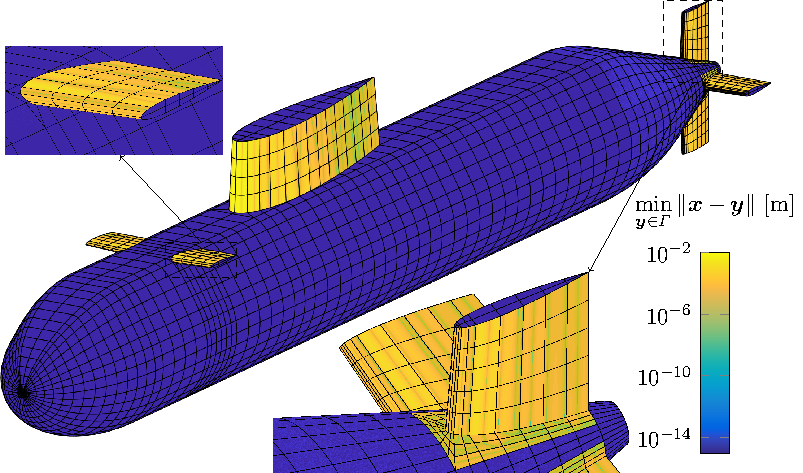
\includegraphics{colorbar}
	\caption{\textbf{An analysis suitable BeTSSi submarine}: The geometric surface approximation $\Gamma_{\check{p}}$ approximates the surface of the exact representation of the BeTSSi submarine $\Gamma$. Surface visualization of the mesh and geometric error for $\check{p}=2$. Most parts of the approximation are exact to machine epsilon precision.}
	\label{Fig3:geometricError}
\end{figure}
\begin{figure}
	\centering    
	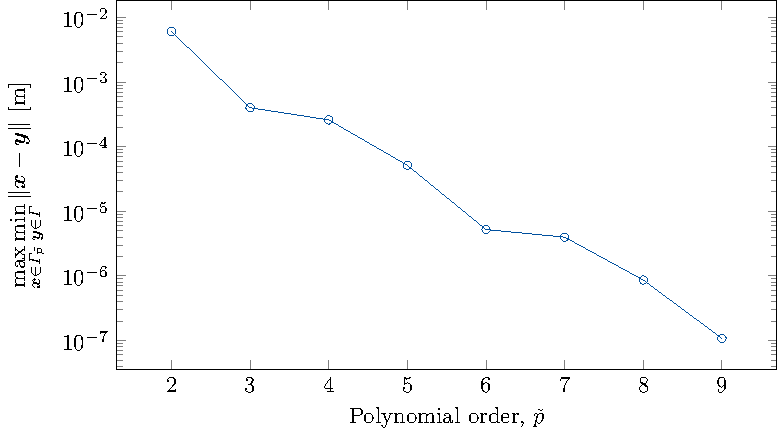
\includegraphics{geometryErrors}
	\caption{\textbf{An analysis suitable BeTSSi submarine}: The geometric surface approximation $\Gamma_{\check{p}}$ approximates the surface of the exact representation of the BeTSSi submarine $\Gamma$. Convergence plot showing exponential convergence to the exact geometry $\Gamma$.}
	\label{Fig3:geometricErrorsL2_1}
\end{figure}
\begin{figure}
	\centering    
	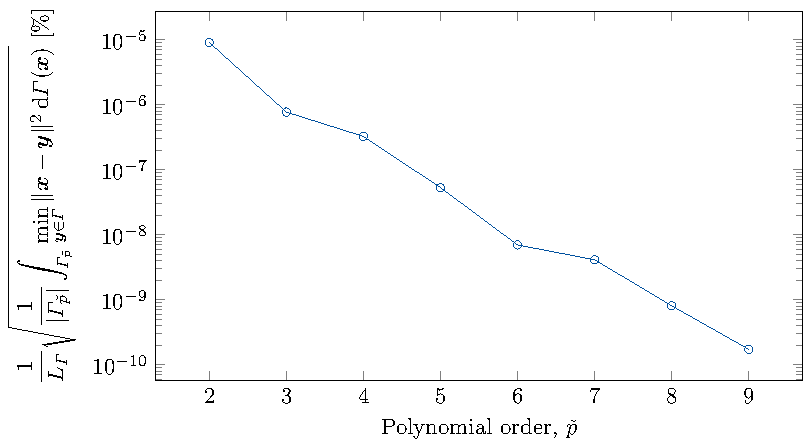
\includegraphics{geometryErrors_2}
	\caption{\textbf{An analysis suitable BeTSSi submarine}: Same as \Cref{Fig3:geometricErrorsL2_1} but in another norm. Here, the characteristic length of the geometry is given by $L_\Gamma = a+L+g_2+g_3$.}
	\label{Fig3:geometricErrorsL2_2}
\end{figure}
\begin{figure}
	\centering    
	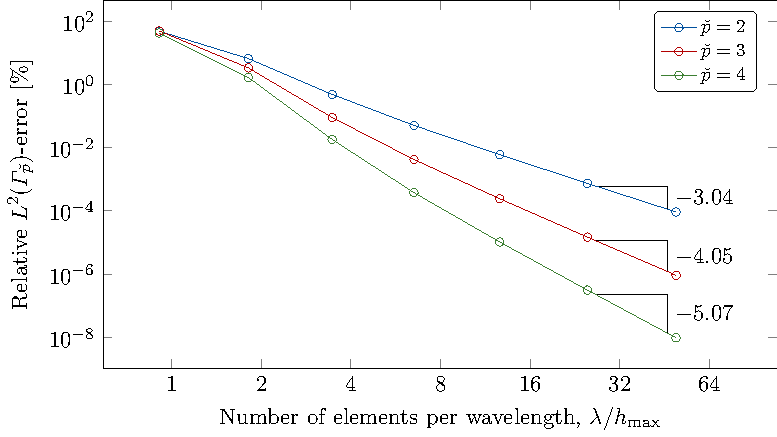
\includegraphics{BCA_P_BA}
	\caption{\textbf{An analysis suitable BeTSSi submarine}: Error of the best approximation for the manufactured solution presented in \Cref{Subsec3:manufactured} on $\Gamma_{\check{p}}$.}
	\label{Fig3:BCA_P_BA}
\end{figure}

\section{Triangulation of the BeTSSi submarine}
\label{Sec3:BeTSSi_triangulation}
Triangularized versions of the exact BeTSSi submarine in \texttt{.stl} (both ASCII and binary) and \texttt{.bdf} format can be found in~\cite{Venaas2019bts} where the triangulations is an optimization of meshes created in \COMSOL (surface mesh corresponding to the \COMSOL volume meshes considered in this work). 
An overview of the triangularization meshes can be found in \Cref{Tab3:BeTSSiTriangularization}. Since these meshes are used by WTD in the simulations they have provided for this work, they are denoted by ${\cal M}_m^{\textsc{wtd}}$.
\begin{table}
	\centering
	\caption{\textbf{Triangularization of the BeTSSi submarine}: Data for the meshes.}
	\label{Tab3:BeTSSiTriangularization}
	\begin{tabular}{c S[table-format = 8.0] S[table-format = 8.0] S[table-format = 1.3,round-mode=places,round-precision=3] S[table-format = 1.3,round-mode=places,round-precision=3] S[table-format = 3.1,round-mode=places,round-precision=1] S[table-format = 1.4,round-mode=places,round-precision=4]}
		\toprule
		Mesh & {\# triangles} & {\# vertices}  & {$h_{\mathrm{max}}^{(1)}$ [$\si{m}$]}  & {$h_{\mathrm{max}}^{(2)}$ [$\si{m}$]}  & {$R_{\mathrm{max}}$} & {$S_{\mathrm{min}}$}\\
		\hline
		${\cal M}_{1}^{\textsc{wtd}}$ & 4140 & 2072 & 2.10916 & 1.89333 & 28.4006 & 0.0336305\\
		${\cal M}_{2}^{\textsc{wtd}}$ & 10406 & 5205 & 1.03183 & 1.00496 & 56.742 & 0.0168107\\
		${\cal M}_{3}^{\textsc{wtd}}$ & 31104 & 15554 & 0.542723 & 0.498592 & 105.253 & 0.00906949\\
		${\cal M}_{4}^{\textsc{wtd}}$ & 106888 & 53446 & 0.280763 & 0.256928 & 202.497 & 0.00471578\\
		${\cal M}_{5}^{\textsc{wtd}}$ & 400886 & 200445 & 0.138583 & 0.130041 & 401.21 & 0.00238013\\
		${\cal M}_{6}^{\textsc{wtd}}$ & 1584014 & 792009 & 0.0722726 & 0.0691461 & 807.597 & 0.00118243\\
		\bottomrule
	\end{tabular}
\end{table}
The \textit{resolution} (res) parameter $\lambda/h_{\mathrm{max}}^{(2)}$ (at $f = \SI{1}{kHz}$) is used in the file names. In~\Cref{Tab3:BeTSSiTriangularization}, $h_{\mathrm{max}}^{(1)}$ is defined as the maximum of the diameters of the smallest circle that inscribes the triangular element. For the $i^{\mathrm{th}}$ triangle with side lengths $l_{i,1}$, $l_{i,2}$ and $l_{i,3}$, it is given by
\begin{equation*}
	h_{\mathrm{max}}^{(1)} = \max_i\frac{2l_{i,1}l_{i,2}l_{i,3}}{\sqrt{(l_{i,1}+l_{i,2}+l_{i,3})(l_{i,1}+l_{i,2}-l_{i,3})(l_{i,1}+l_{i,3}-l_{i,2})(l_{i,2}+l_{i,3}-l_{i,1})}}.
\end{equation*}
\COMSOL uses another common definition of the element size, namely the largest side length of the triangle
\begin{equation*}
	h_{\mathrm{max}}^{(2)} = \max_{i,j} l_{i,j}.
\end{equation*}
The three angles of a triangle may be computed by
\begin{equation*}
\begin{aligned}
	\alpha_{i,1} &= \cos^{-1}\left(\frac{l_{i,2}^2+l_{i,3}^2-l_{i,1}^2}{2l_{i,2}l_{i,3}}\right),\quad
	\alpha_{i,2} = \cos^{-1}\left(\frac{l_{i,1}^2+l_{i,3}^2-l_{i,2}^2}{2l_{i,1}l_{i,3}}\right)\\
	\alpha_{i,3} &= \cos^{-1}\left(\frac{l_{i,1}^2+l_{i,2}^2-l_{i,3}^2}{2l_{i,1}l_{i,2}}\right),
\end{aligned}
\end{equation*}
such that the maximum and minimum angle are given by
\begin{equation*}
	\alpha_{\mathrm{max}} = \max_{i,j}\alpha_{i,j}\quad\text{and}\quad\alpha_{\mathrm{min}} = \min_{i,j}\alpha_{i,j},
\end{equation*}
respectively. The maximum aspect ratio is defined by
\begin{equation*}
	R_{\mathrm{max}} = \max_i \frac{\max_j l_{i,j}}{\min_j l_{i,j}}
\end{equation*}
and the minimum skewness is defined by
\begin{equation*}
	S_{\mathrm{min}} = \min_{i,j}\left[1-\max\left(\frac{\alpha_{i,j}-\alpha_{\mathrm{e}}}{\ang{180}-\alpha_{\mathrm{e}}}, \frac{\alpha_{\mathrm{e}}-\alpha_{i,j}}{\alpha_{\mathrm{e}}},\right)\right], \quad\alpha_{\mathrm{e}}= \ang{60}.
\end{equation*}
The main take-away here is the inevitability of the increase in the aspect ratio (and the reduction in skewness) during refinement. This is because of the presence of non-Lipschitz domains.